\documentclass{scrartcl}

\usepackage{siunitx}
\usepackage{graphicx}
\usepackage{caption}
\usepackage{glossaries}
\usepackage[english]{babel}
\usepackage{booktabs}
\usepackage[linktoc=all,hidelinks]{hyperref}
\usepackage{fontspec}
% \usepackage{authblk}
\usepackage{unicode-math}

% \makeatletter
% \renewcommand\AB@affilsepx{,~ \protect\Affilfont}
% \makeatother

\setkomafont{author}{\sffamily}

\newcommand{\nump}[2]{\num[round-mode=places,round-precision=#2]{#1}}
\DeclareGraphicsExtensions{.pdf,.eps}
\bibliographystyle{unsrt}

\title{Project Proposal}
\subtitle{A study of machine learning algorithms for reconstruction of missing energy in particle physics experiments.}
% \subject{Statistical Machine Learning}

\author{
  Max Isacson, \url{max.isacson@physics.uu.se}
  \and
  Mikael M\aa rtensson, \url{mikael.martensson@physics.uu.se}
  \and
  Camila Rangel Smith, \url{camila.rangel@physics.uu.se}
  \and
  Henrik Öhman, \url{ohman@cern.ch}
}
% \author[1]{Max Isacsson}
% \author[2]{Mikael M\aa rtensson}
% \author[3]{Camila Rangel Smith}
% \author[4]{Henrik \"{O}hman}
% \affil[1]{\small\url{max.isacsson@physics.uu.se}}
% \affil[2]{\url{mikael.martensson@physics.uu.se}}
% \affil[3]{\url{camila.rangel@physics.uu.se}}
% \affil[4]{\url{ohman@cern.ch}}

\newacronym{ANN}{ANN}{Artificial Neural Network}

\newcommand{\etmiss}{$E_\mathrm{T}^\text{miss}$}
\newcommand{\exmiss}{$E_x^\text{miss}$}
\newcommand{\eymiss}{$E_y^\text{miss}$}

\begin{document}
\maketitle

\begin{figure}
    \centering
    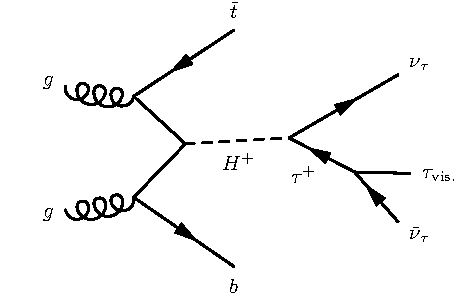
\includegraphics[width=.7\textwidth]{img/heavyHplustaunu4fs.pdf}
    \caption{Feynman diagram of the production and decay of a charged Higgs boson. Not shown is the hadronic top decay $\bar t \to \bar b W^-(q \bar q')$.}\label{fig:hplus}
\end{figure}

\section{Background}
\subsection{Hadron collider experiments}
At particle colliders two beams of hadrons\footnote{Hadrons are non-elementary particles consisting quarks, which are elementary, and held together by the strong force, which is mediated by glouns. Examples of hadrons are the proton and the neutron.} are accelerated to relativistic speeds and and collided head-on. The quarks and gluons in the hadrons interact, producing all kinds of elementary and non-elementary particles. Due to mass conservation, the mass of the created particle cannot exceed the combined energy of the collision. Most particles produced in the interaction are highly unstable and quickly decays to more stable ones. The properties of these short-lived particles has to be deduced by their decay products.

General purpose detectors are used to characterize the reaction products. Moving from the collision point outwards, the detectors consists of: a tracker placed inside a magnetic field that measures the track and momentum of charged particles; an electromagnetic calorimeter which measures the energy of photons and electron; a hadronic calorimeter that measured the energy of hadrons, and a muon chamber that detects muons (a heavier cousin to the electron) which are not stopped by the calorimeters. The only particles not detected are the elusive neutrinos, which instead show up as missing energy.

\subsection{The charged Higgs boson}
The charged Higgs boson is a hypothesized particle that is present in some extensions of the Standard Model. The charged Higgs boson can be either heavier or lighter than the top quark. Here we consider its heavy form, in which it is produced from two gluons in particle collisions, and in association with a top and a bottom quark, figure \ref{fig:hplus}. The two main decays of the charged Higgs boson are decays to a top and a bottom quark ($H⁺→tb$), and decays to a tau lepton and a neutrino ($H⁺→τν$). The charged Higgs boson decay into a tau lepton and a neutrino offers a clean signature that is relatively easy to discriminate against background events.

The tau lepton in turn either decays to a light lepton (electron or muon) and two neutrinos, or to hadrons (charged and neutral pions) and one neutrino. Here we consider hadronically decaying tau leptons.

The components of the event final state (in regard to the production and decay mode), which also form the base of our set of input variables, are the top and bottom quark from the associated production, the visible component of the hadronically decaying tau lepton, and the missing energy.

\subsection{Missing energy}
The neutrinos in the charged Higgs boson decays only interact with matter via the weak interaction. Since the this interaction is (as its name suggests) weak, neutrinos will travel through the detector without affecting the matter that constitues it. The neutrinos can therefore only be detected in form of the absence of interaction. This absence is called missing energy.

Furthermore, since the particle beam consists of composite objects (protons) as apart from point-like objects (e.g. electrons), it is not possible to know how large portion of the beam particles' momentum go into the production of the charged Higgs boson. Therefore we can only make use of the energy and momentum conservation constraints in the directions transverse to the beam (x and y). For detected particles, the momentum can be reconstructed in all three spatial directions, while for the neutrinos this information is completely unknown. In the end we are left with two quantities: \exmiss\ and \eymiss.

The neutrino from the hadronic tau decay only carries a small amount of the energy of the tau lepton. A good approximation is to disregard this neutrino, and assume that all missing energy comes from the neutrino originating from the charged Higgs boson decay. This simplifies the event topology, and thus the statistical model, by removing one unknown variable.

\section{The Dataset}
\subsection{Structure}
The dataset consists of simulated $pp$ collision events, in which a charged Higgs is produced and decays as $H^+\to\tau\nu$. Each event is described by one set of observable variables and one set of unobservable variables.

Observable variables:
\begin{itemize}
    \item \exmiss, \eymiss --- The $x$- and $y$-components of the missing energy.
    \item $P_{\tau_\mathrm{vis.}}$ --- The 4-momentum of the visible (hadronic) part of the $\tau$ decay.
    \item $P_{b_0}$, $P_{b_1}$, $P_{q_0}$, $P_{q_1}$ --- The 4-momenta of the two $b$-jets and two light jets.
\end{itemize}

Unobservable variables:
\begin{itemize}
    \item $P_{\nu_\tau}$ --- The 4-momentum of the neutrino from the charged Higgs decay.
    \item $P_{\bar\nu_\tau}$ --- The 4-momentum of the neutrino from the $\tau$ decay.
\end{itemize}

\subsection{Production}
MG5\_aMC@NLO \cite{Alwall:2014hca} is used for the matrix element computation of $gg / q \bar q \to H^+$ and the event simulation. The events are then passed to PYTHIA8 \cite{Sjöstrand2015159} for the showering and hadronization, and for the $H^+\to \tau\nu$ decay. Finally, the detector response is simulated using DELPHES \cite{Favereau2014} with an ATLAS-like geometry.

\subsection{Estimated and true quantities}
The true quantities for both the observable and the unobservable variables are available as output from the event simulation. The estimated values for the observable variables are reconstructed from the output from the detector response simulation.

\section{Solution strategy}
A number of machine learning algorithms will be compared for this regression problem. Specifically we will compare artificial neural networks, Bayesian regression, support vector regression, and the Gaussian process. The algorithms will principally be judged based on the resolution of the reconstructed transverse (perpendicular to the beam axis) component of the missing energy. The ability to reconstruct the component of the missing energy in the longitudinal direction (parallel to the beam axis) will also be investigated.

The estimated (reconstructed) observable quantities are used as inputs to the training, while the true quantities for the \exmiss, \eymiss, $P_{\nu_\tau}$, and $P_{\bar\nu_\tau}$ are used as target values.

\bibliography{refs}

\end{document}
